%%%%%%%%%%%%%%%%%%%%%%%%%%%%%%%%%%%%%%%%%%%%%%%%%%%%%%%%%%%%%%%%%%%%%%%%%%%%%%%
%%%%%%%%%%%%%%%%%%%%%%%%%%%%%%%%%%%%%%%%%%%%%%%%%%%%%%%%%%%%%%%%%%%%%%%%%%%%%%%
%%%%%%%%%%%%%%%%%%%%%%%%%%%%%%%%%%%%%%%%%%%%%%%%%%%%%%%%%%%%%%%%%%%%%%%%%%%%%%%
\section{Implementation}
SOSflow's core routines allow it to:
%
\begin{enumerate}
      %
    \item Facilitate on-line capture of data from many sources.
      %
    \item Annotate the gathered data with context and meaning.
      %
    \item Store the captured data on node in a way that can be
      searched with dynamic queries in real-time as well as being
      suitable for aggregation and long-term archival.
      %
\end{enumerate}
%%%%%
SOSflow is divided into several components.  The core components are:
%
\begin{itemize}
      %
    \item \textbf{libsos} - Library of common routines for interacting with
      sosd daemons and SOS data structures
      %
    \item \textbf{sosd(listener)} - Daemon process running on each node
      %
    \item \textbf{sosd(db)} - Daemon process running on dedicated resources
      that stores data aggregated from one or more in situ daemons
      %
    \item \textbf{sosa} - Analytics framework for online query of SOS data
      %
\end{itemize}

\subsection{Architecture Overview} %------------------------------------------%
%%%%%
\begin{figure}[h]
  \centering
  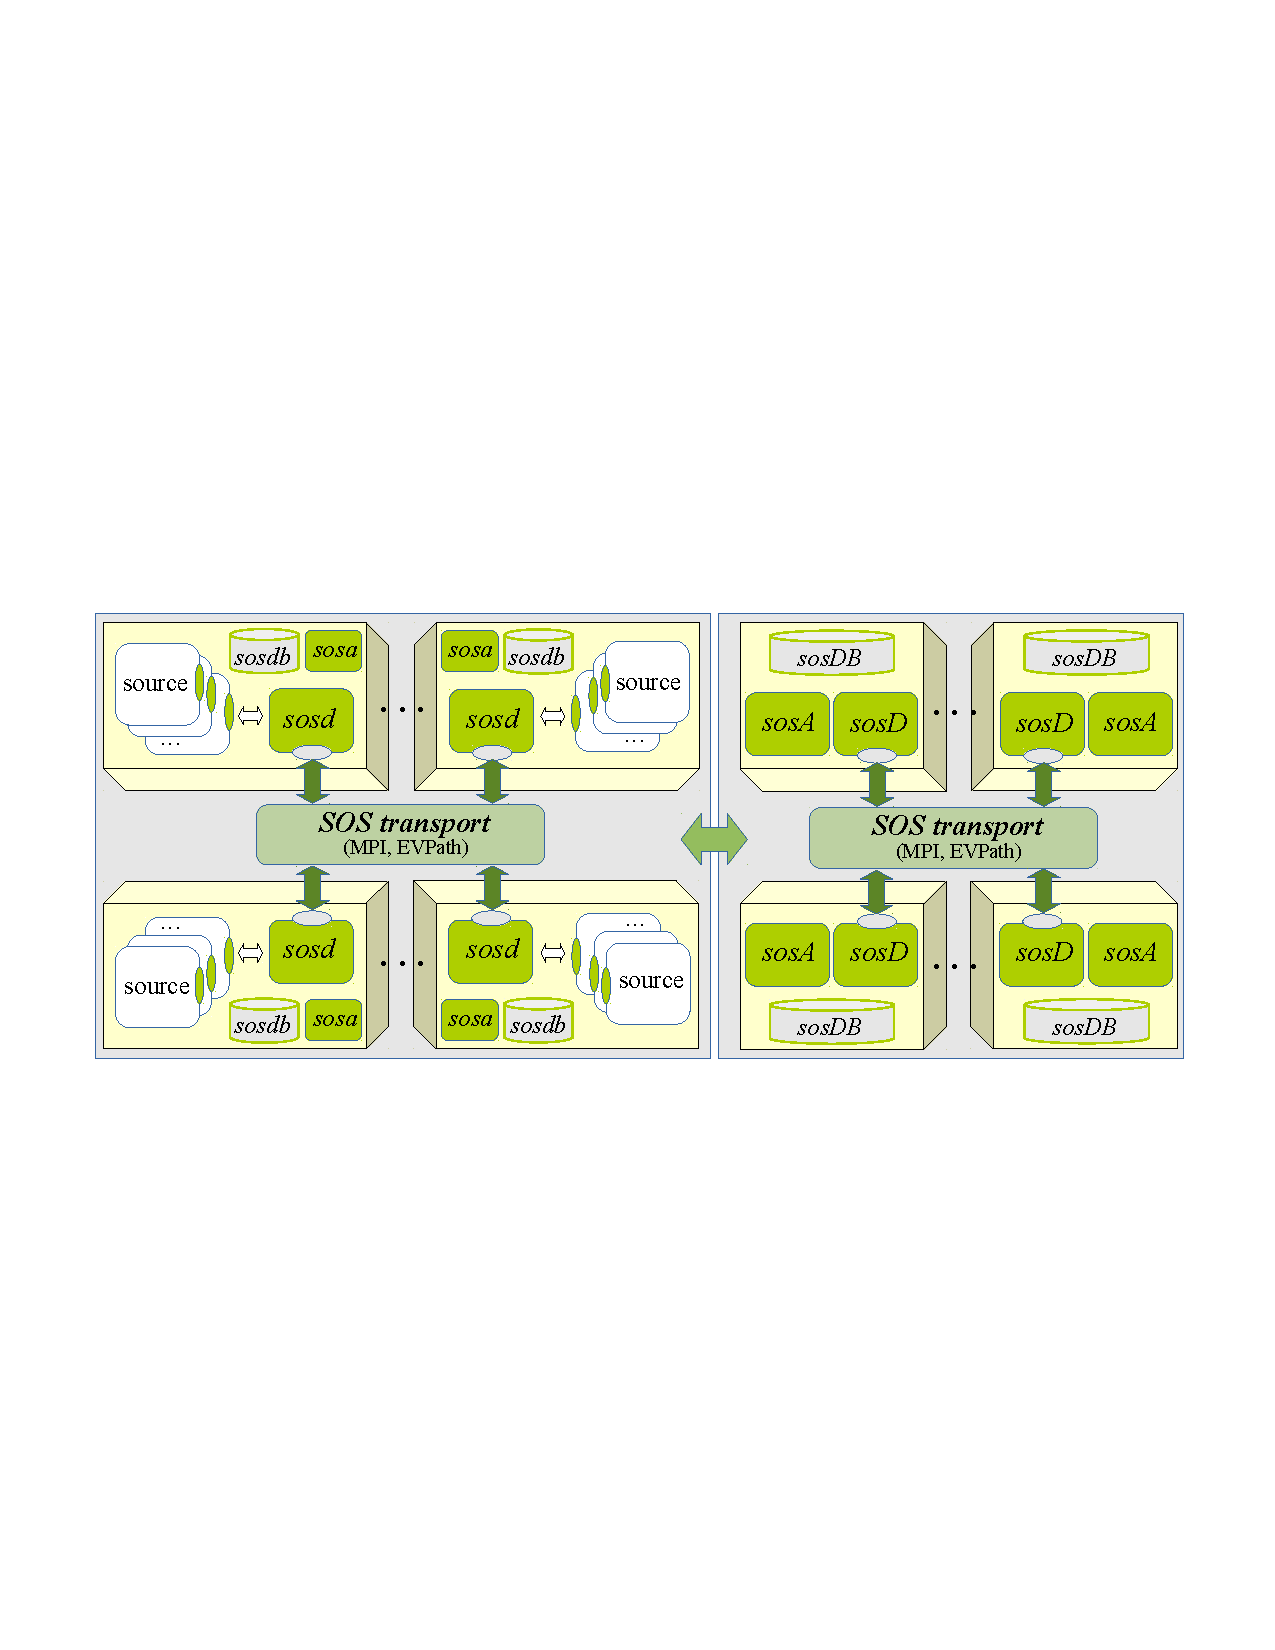
\includegraphics[width=\columnwidth]{images/sos.pdf}
  \caption{SOSflow Internal Topology}
  \label{fig_sos_topology}
\end{figure}
%%%%%


%%%%%
\begin{figure}[h]
\centering
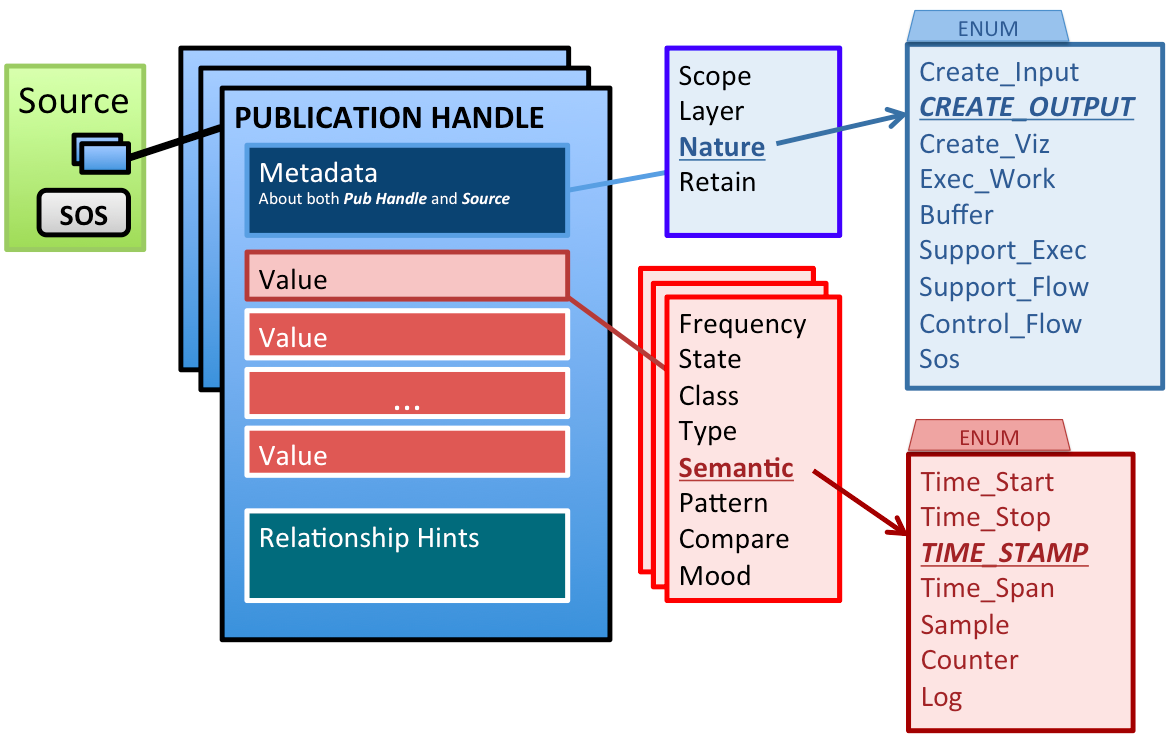
\includegraphics[width=\columnwidth]{images/pub_handle.png}
\caption{Structure of an SOS Publication Handle}
\label{fig_pub_handle}
\end{figure}
%%%%%

%%%%%
Data in SOSflow is stored in a ``publication handle'' object.
%
This object organizes all of the application context information and
value-specific metadata, as well as managing the history of updates to
a value pending pending transmission to a sosd(listener), called
\textit{value snapshots}.
%
Every value that is passed through the SOSflow API is preserved and
eventually stored in a searchable database, along with any updated
metadata such as its timestamp tuples.
%
Multiple updates to the same value prior to a call to SOS\_publish()
are no exception.
%
Prior value snapshots are queued up and faithfully transmitted along
with the most recent update to that value.
%%%%%
%%%%%
\begin{figure}[h]
\centering
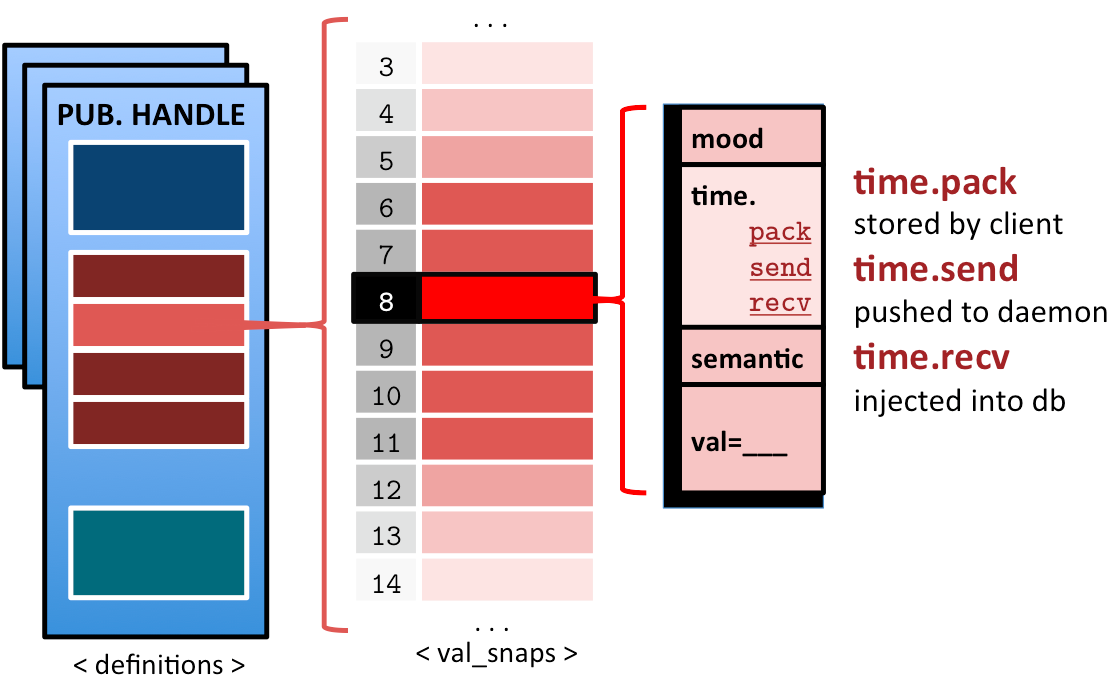
\includegraphics[width=\columnwidth]{images/val_snaps.png}
\caption{Complete History of For All Values, Including Metadata}
\label{fig_val_snaps}
\end{figure}
%%%%%
%
\par
%
The SOSflow runtime utilizes different information transport methods
where appropriate.
%
Communication between client applications and their on-node daemon
takes place over a TCP socket connection.
%
%%%%%
\begin{figure}[h]
\centering
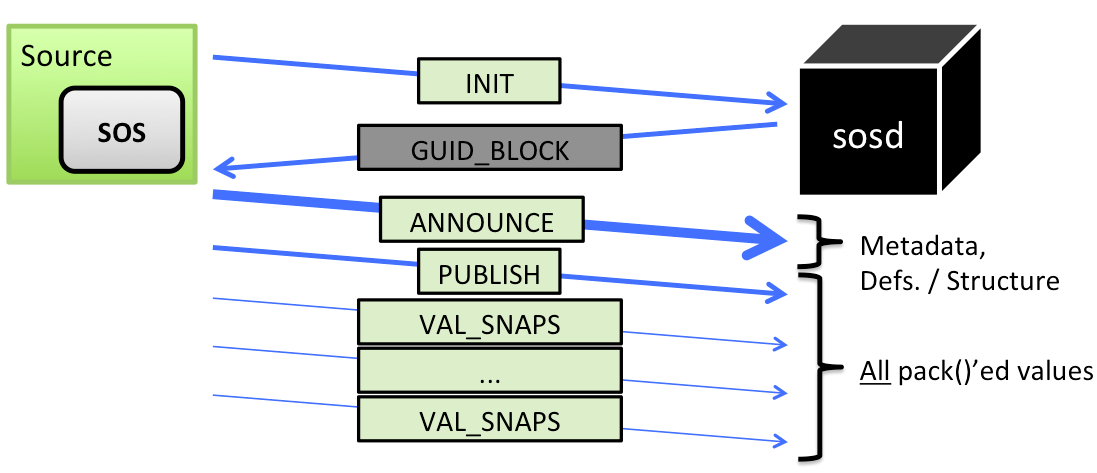
\includegraphics[width=\columnwidth]{images/sosd_protocol.png}
\caption{In Situ Client/Daemon Communication Protocol}
\label{fig_sosd_protocol}
\end{figure}
%%%%%
%
Messages are read off the socket rapidly and placed in the daemon's
unbounded asynchronous thread-safe queues to be processed by the
daemon's local\_sync and cloud\_sync threads.
%
The socket is nearly immediately clear for the next queue'd message to
be received, and an example of the consistent rate of message uptake
despite variable message injection rates is discussed in the Results
section.
%
Once a message is transmitted to the SOSflow daemon, it is placed in
an asynchronous queue for storage into an on-node database.
%
The same message is enqueued for transmission to an off-node data
aggregation target.
%
The SOSflow runtime uses MPI and the high-speed interconnect network
of the HPC machine when transmitting information off-node.
%%%%
\begin{figure}[h]
  \centering
  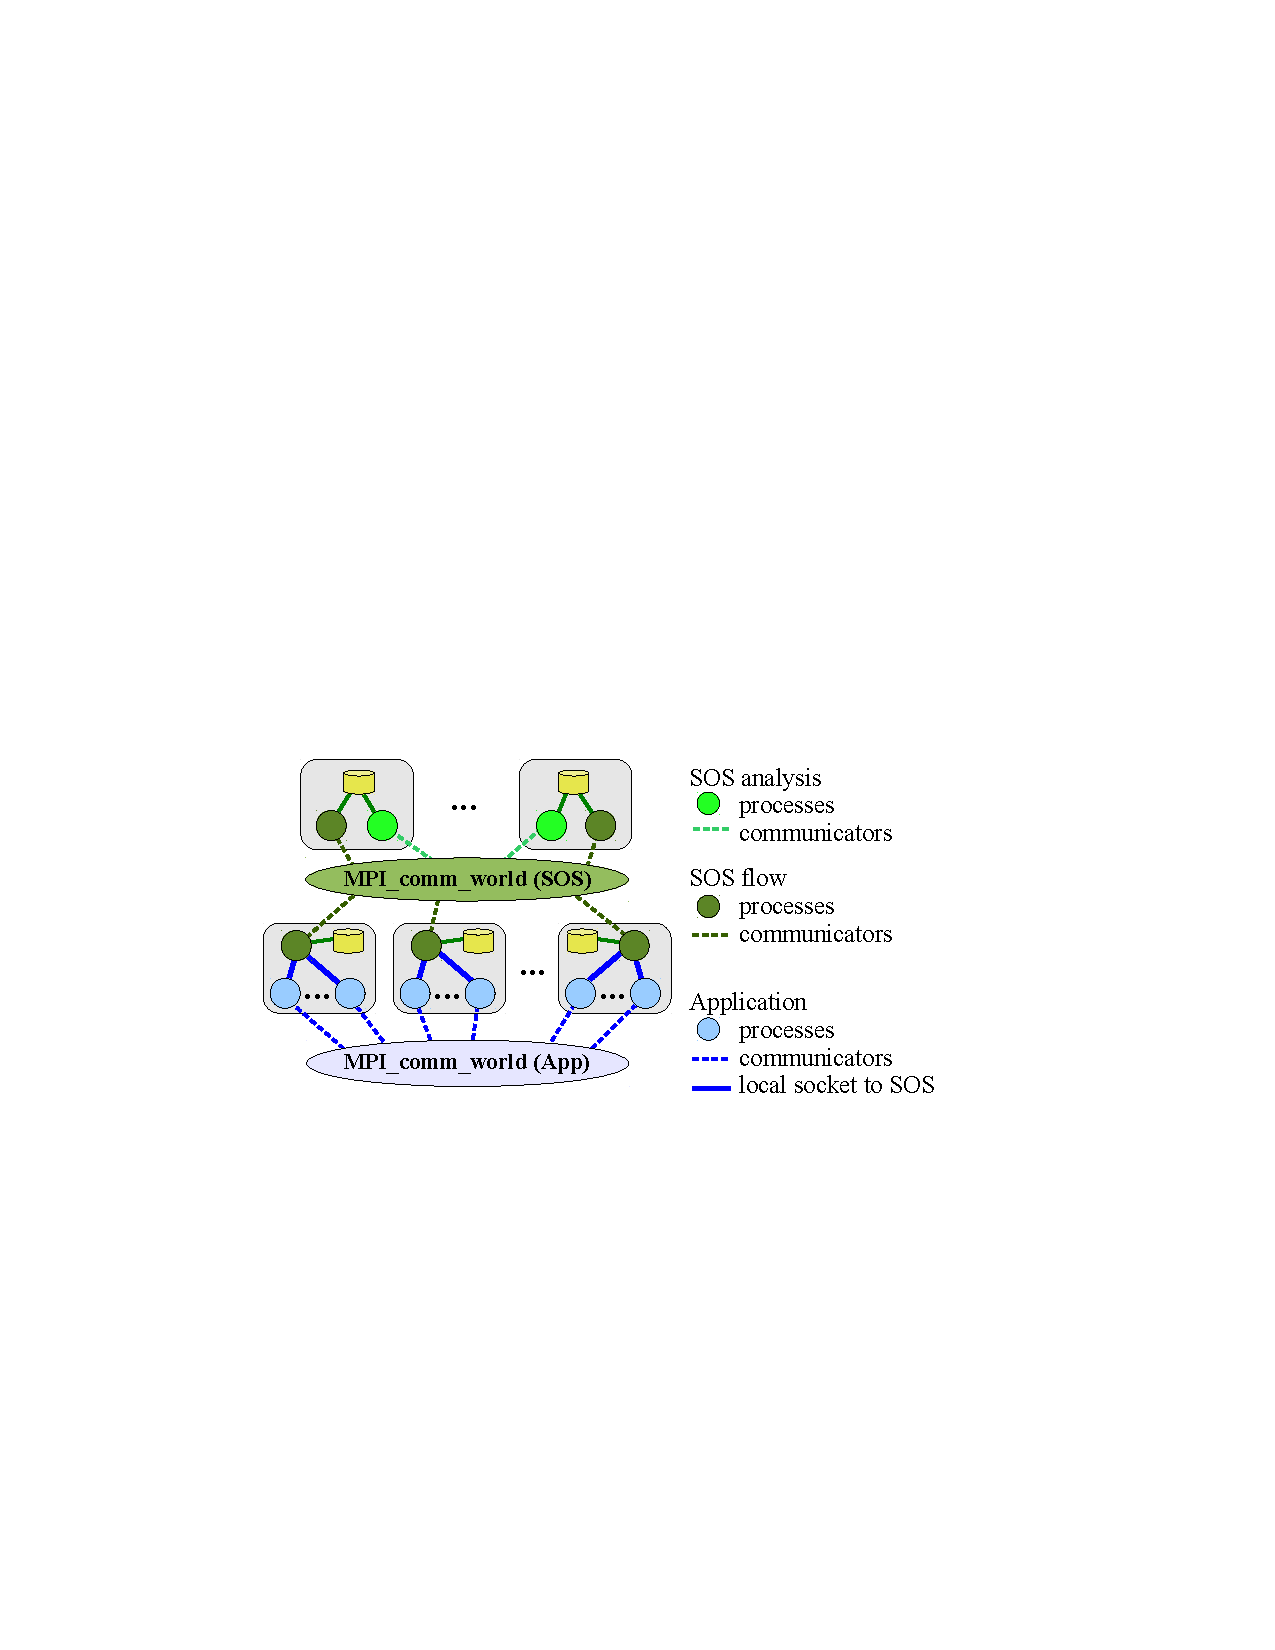
\includegraphics[width=\columnwidth]{images/sos-mpmd.pdf}
  \caption{SOSflow Communicates w/MPI and Sockets}
  \label{fig_sos_mpmd}
\end{figure}
%%%%%
%
SOSflow does not participate in the MPI communicator[s] of the
applications that it is monitoring, so no special integration
programming is required of application developers who use MPI or
sockets in their code.
%
\par
%
%
\subsection{Library: libsos} %------------------------------------------------%
%
Applications that make direct use of SOSflow through its API are called
\textit{clients}.
%
Clients must link in the libsos library which provides them with all of
the data structures and routines essential for interacting with
the SOSflow runtime platform.
%
The library routines are thread safe, and no process-wide state is
maintaned within the library, allowing the pieces of a process
comprising multiple libraries and application parts to interact with
SOSflow independently of each other.
%
\par
%%
The primary interaction between a client and SOSflow is through the
publication handle (pub).
%
When a client initializes its SOSflow instance, it communicates with the
daemon and obtains a set of global unique ID (guid) tags.
%
Clients pack values into a pub and they are automatically assigned a guid.
%
When the client publishes that handle, all values and transmitted to
the SOSflow on-node daemon, including the complete history of each
value's updates from the last to the present publish call.
%
\par
%
All of the communication functions in the sos client library are
handled transparently, SOSflow users need only interact with a simple API
to define and store values that they can then publish up to the daemon
as appropriate.
%
The protocols and the codes of the client library are designed to be
fast and minimize resource usage, though they will buffer values for
the user if they choose to hold them and only transmit to the daemon
at intervals.
%
\par
%
Communication with the sosd(listener) is always initiated by the
clients when they call SOS_publish() on a publication handle.
%
Client applications do not need to monitor a socket, though certain
SOS client roles can spawn a lightweight background thread that
periodically checks in with their local daemon to see if any feedback
has been sent to that application, allowing for run-time adaptivity to
be decoupled from the application's schedule for transmitting its
information to SOSflow.


\subsection{Daemon: sosd(listener)} %-----------------------------------------%
The sosd daemon is itself an MPI application, and it is launched as a
background process in user space at the start of a job script, before
the scientific workflow begins.
%
The daemons first go through a coordination phase where they each
participate in an MPI\_Allreduce() with all other daemon ranks in
order to share their role (DAEMON, DB, or ANALYTICS) and the name of
the host they are running on.
%
During the coordination phase, listener daemons select the sosd(db)
aggregate database that they will target for automatic asynchronous
transfer of the data they capture.

\subsection{Database: sosd(db)} %---------------------------------------------%
%
SOSD(db) uses the open-source SQLite database engine for its on-node
database.
%
At the time of this writing, SQLite technology is also used for the
aggregate databases, though it is anticipated that an interface to the
Cassandra database will be used for that role.
%
\par
%
SQLite databases are lightweight, fast, and flexible, suitable for
streaming values into with very low overhead.


\subsection{Analytics: sosa} %------------------------------------------------%
%
SOSflow analytics modules are independent programs that are launched
and operate alongside the SOSflow run-time.
%
The primary role of the analytics modules is to query the database
and produce functional output such as real-time visualizations of
performance metrics, steering commands to facilitate optimizations, or
global resource bound calculation and policy enforcement.
%
The modules can be deployed in a distributed fashion to run on the nodes
where the applications are executing, or they can be deployed on dedicated
resources and coupled with the aggregate databases for fast queries
of the global state.
%
Analytics modules are encouraged to make use of the high-speed
interconnect of the HPC machine in order to share data amongst themselves.
%
\par
%
SOSflow provides an API for client applications to register
a callback function to a named trigger.
%
Those triggers can to be fired off by analytics modules, and arbitrary
data structures can be passed to the triggered functions.
%
Triggers may be fired for a specific single process on one node,
or for an entire node, or an entire scientific workflow.



%%%%%
%%%
%%%  EOF
%%%
